\documentclass[12pt,a4paper,titlepage,AutoFakeBold]{article}
%設定頁面
\textwidth 170mm %文寬
%\textheight 260mm %文長
%\topsep -20mm \headsep -20mm %調整頁頭大小,可以是負值
%\hoffset -40pt
\usepackage{geometry}
\geometry{left=2cm=right,top=2.5cm=bottom}

%Typesetting

%about font shape
\usepackage{fontspec}
%\setmainfont{P22MayflowerPro}
\newcommand{\bt}[1]{%
    \begin{center}{\Large\textbf{#1}}\end{center}}
\newcommand{\bfit}[1]{%
    \textbf{\textit{#1}}}
\newcommand{\bfup}[1]{%
    \textbf{\textup{#1}}}
\newcommand{\mbf}[1]{%
    \textbf{\mathbf{#1}}}
\usepackage{type1cm}

\usepackage{xeCJK} 
\setCJKmainfont{DFKaiShu-SB-Estd-BF}
\newCJKfontfamily\Kai{DFKaiShu-SB-Estd-BF} 
\newCJKfontfamily\lie{STLibianTC-Regular}
\XeTeXlinebreaklocale "zh"   
\XeTeXlinebreakskip = 0pt plus 1pt %設定中文
%\renewcommand\contentsname{目錄}

\usepackage[shortlabels]{enumitem}
%\usepackage{enumerate}

%about section
%\renewcommand{\thesection}{\Roman{section}.} 
%\renewcommand{\thesubsection}{\Roman{subsection}.} 
\setcounter{section}{1}
\setcounter{subsection}{1}

%color
\usepackage[dvipsnames]{xcolor}
\definecolor{yel}{RGB}{240,200,90}
\definecolor{3b1bblue}{RGB}{106,177,198}
\definecolor{3b1bred}{RGB}{220,100,90}
\definecolor{Green}{RGB}{50,180,30}
%\pagecolor{backgroud}
%\color{black}

%縮排
\usepackage{indentfirst}
\parindent=0pt 

%頁首、尾文字
\usepackage{fancyhdr}
\pagestyle{fancy}
\chead{}
\lhead{}
\rhead{}
\lfoot{}
\cfoot{\thepage}
\rfoot{}
\newcommand{\fancy}[2]{%
    \lfoot{LECTURE #1. #2}\rhead{Lec #1}}
\renewcommand{\headrulewidth}{0pt} %上線寬
%\renewcommand{\footrulewidth}{0.4pt} %下線寬
%\renewcommand{\abstractname}{Executive Summary}
%\renewcommand{\chaptername}{}

% Math and some symbol
\usepackage{amsmath, amsthm, xfrac, amssymb}
\DeclareMathOperator{\Area}{Area}
\DeclareMathOperator{\grad}{grad}
\DeclareMathOperator{\curl}{curl}
\DeclareMathOperator{\ord}{ord}
\DeclareMathOperator{\Sp}{span}
\DeclareMathOperator{\nsp}{Null}
\DeclareMathOperator{\csp}{Col}
\DeclareMathOperator{\rsp}{Row}
\DeclareMathOperator{\rk}{rank}
\DeclareMathOperator{\nul}{nullity}
\DeclareMathOperator{\rref}{rref}
\DeclareMathOperator{\im}{Im}
\DeclareMathOperator{\diag}{diag}

\newcommand{\re}{\mathbb{R}}
\newcommand{\na}{\mathbb{N}}
\newcommand{\inte}{\mathbb{Z}}
\newcommand{\eucl}{\mathbb{E}}
\newcommand{\ra}{\mathbb{Q}}
\newcommand{\comp}{\mathbb{C}}
\newcommand{\rs}{{\color{red}$\star$}}
\newcommand{\normal}{\trianglelefteq}
\newcommand{\action}{\circlearrowright}



\usepackage{pifont}
\newcommand{\cmark}{\ding{51}}
\newcommand{\xmark}{\ding{55}}
\newcommand{\uxm}{\textup{\ding{55}}}
\newcommand{\cirnum}[1]{%
    \ding{\numexpr171+#1\relax}}
\newcommand{\Qed}{%
    \null\nobreak\hfill\ensuremath{\square}}

% defined integral
\newcommand{\Value}[1]{%
    \left.{#1}\phantom{\Big|}\right|}

%very nice
\usepackage{nicematrix}

\usepackage{cancel}
%\usepackage[thicklines]{cancel}
\newcommand{\Ccancel}[2][3b1bblue]{%
    \renewcommand\CancelColor{\color{#1}}\cancel{#2}}
\newcommand{\Dcancel}[2][red!70]{%
    \renewcommand\CancelColor{\color{#1}}\cancel{#2}}
\newcommand{\Ecancel}[2][black]{%
    \renewcommand\CancelColor{\color{#1}}\cancel{#2}}

\newcommand{\red}[1]{%
    {\color{red!70}{#1}}}

\usepackage{mathrsfs} %English Calligraphy
\usepackage{bm} % 數學粗體

\usepackage{soul}
\setul{0.5ex}{0.2ex}
\setulcolor{red}
% underline with red color

\usepackage{tikz,tikz-cd}
\tikzset{R/.style={circle, draw, white, fill=red!80, minimum size=10mm}}
\tikzset{B/.style={circle, draw, white, fill=black!80, minimum size=10mm}}
\tikzset{C/.style={circle, draw}}
\tikzset{
    level 1/.style={sibling distance=18em, level distance=3em},
    level 2/.style={sibling distance=5em, level distance=3em},
    level 3/.style={sibling distance=4em, level distance=3em},
}

\usepackage{mathtools}
%\newcommand{\verteq}{\rotatebox{90}{$\,=$}}
%\newcommand{\equalto}[2]{\underset{\scriptstyle\overset{\mkern4mu\verteq}{#2}}{#1}}
\newcommand{\veq}{\mathrel{\rotatebox{90}{$=$}}}
\newcommand{\vneq}{\mathrel{\rotatebox{90}{$\neq$}}}
\usepackage{extarrows} % arrow with text
\newcommand{\litrom}[1]{%
    \romannumeral#1}
\newcommand{\caprom}[1]{%
    \uppercase\expandafter{\romannumeral#1}}
%羅馬數字

\newtheorem{thm}{Theorem}
\newtheorem*{lemma}{Lemma}
\newtheorem{corollary}{Corollary}

\setcounter{page}{1}
%\pagenumbering{roman}
%\pagestyle{plain}
%設定頁碼

%simply box
\usepackage{varwidth}
\setlength{\fboxrule}{0.6pt}
\newcommand{\varbox}[1]{%
    \fbox{\varwidth{\linewidth}#1\endvarwidth}}

%%%%%%%%%%%%%%%%%%%%%%%%%%%%%%%%%%%%%%%%%%
\newcounter{prop} 
\setcounter{prop}{3}
\renewcommand{\theprop}{\arabic{prop}}
\newcommand{\prop}{%
    \refstepcounter{prop}{\bf{Proposition \theprop.}}}
\newcommand{\cor}{%
    \refstepcounter{prop}{\bfit{Corollary \theprop. }}}

%Throrem in the box
\usepackage[framemethod=TikZ]{mdframed}
%\mdtheorem{boxdef}{Defintion.}
%\newmdtheoremenv{boxx}[lemma]{Theorem}
%\newmdtheoremenv{lemo}{Lemma}
%\newmdenv{}{}
%Just a box
\newcounter{boxthm} 
\setcounter{boxthm}{0}
\renewcommand{\theboxthm}{\arabic{boxthm}}
\newenvironment{boxthm}[2][]{%
    \refstepcounter{boxthm}
    \mdfsetup{%
        innertopmargin=10pt,%
        innerbottommargin=10pt,%
        linecolor=black,%
        linewidth=0.6pt,topline=true,%
        frametitleaboveskip=\dimexpr-\ht\strutbox\relax}
    \begin{mdframed}
        \textbf{\textit{Theorem#1}}\it\relax%
        \label{#2}
    }{\end{mdframed}}

\newcounter{boxdef} 
\setcounter{boxdef}{0}
\renewcommand{\theboxdef}{\arabic{boxdef}}
\newenvironment{boxdef}[2][]{%
    \refstepcounter{boxdef}
    \mdfsetup{%
        innertopmargin=10pt,%
        innerbottommargin=10pt,%
        linecolor=black,%
        linewidth=0.6pt,topline=true,%
        frametitleaboveskip=\dimexpr-\ht\strutbox\relax
    }
    \begin{mdframed}
        \textbf{\textit{Definition \theboxdef#1}}\it\relax%
    \label{#2}
    }{\end{mdframed}}

\newenvironment{boxx}[1][]{%
    \mdfsetup{%
        innertopmargin=10pt,%
        innerbottommargin=10pt,%
        linecolor=black,%
        linewidth=0.6pt,topline=true,%
        frametitleaboveskip=\dimexpr-\ht\strutbox\relax}
    \begin{mdframed}\relax}{\end{mdframed}}
%%%%%%%%%%%%%%%%%%%%%

% Add graph
\usepackage{import}
\usepackage{xifthen}
\usepackage{pdfpages}
\usepackage{transparent}
\newcommand{\incfig}[1]{%
    \def\svgwidth{\columnwidth}
    \import{/Users/baxiche/Documents/LaTeX/Drawing/}{#1.pdf_tex}
}

\usepackage[titletoc]{appendix}
\renewcommand{\appendixpagename}{Appendix}
\renewcommand{\abstractname}{\textbf{摘要}}
\renewcommand{\contentsname}{\textbf{目錄}}
%\renewcommand{\bibname}{參考文獻}

\usepackage{hyperref}
\hypersetup{
    colorlinks=true,
    linkcolor=blue,
    filecolor=blue,      
    urlcolor=blue,
    citecolor=cyan,
}

%\usepackage[linesnumbered]{algorithm2e}
\usepackage{algorithm2e}
%\usepackage[noend]{algpseudocode}
\SetFuncSty{textsc}
\SetProgSty{textup}
\SetKw{Break}{break}
\SetKw{Conti}{continue}

\usepackage{xpatch}
\xpretocmd{\algorithm}{\hsize=\linewidth}{}{}

\usepackage{listings}
\definecolor{commentgreen}{RGB}{2,112,10}
\definecolor{eminence}{RGB}{108,48,130}
\definecolor{weborange}{RGB}{24,150,100}
%\definecolor{weborange}{RGB}{224,108,117}
\definecolor{frenchplum}{RGB}{129,20,83}

\lstset {
    language=c,
    frame=tb,
    tabsize=4,
    showstringspaces=false,
    numbers=left,
    %upquote=true,
    commentstyle=\color{commentgreen},
    keywordstyle=\color{eminence},
    stringstyle=\color{red},
    basicstyle=\small\ttfamily, % basic font setting
    emph={int,char,double,float,unsigned,void,bool},
    emphstyle={\color{blue}},
    % keyword highlighting
    classoffset=1, % starting new class
    otherkeywords={>,<,.,;,-,!,=,~},
    morekeywords={>,<,.,;,-,!,=,~},
    keywordstyle=\color{weborange},
    classoffset=0,
}

\title{DSA Hw 2}
\author{40840903S 蘇簡宏}
%\date{}
\begin{document}
\fontsize{12pt}{20pt}\selectfont
%\maketitle

DSA hw4

40840903s 蘇簡宏


\section*{Problem 0 - Proper References}
\begin{itemize}[noitemsep]
    \item Problem 1: 李芸芳(B08502041).
    \item Problem 2: all by myself.
    \item Problem 3: all by myself.
    \item Problem 4: all by myself.
\end{itemize}

\newpage 
\section*{Problem 1 - Hash Table and Disjoint Set}
\begin{enumerate}[label=\arabic*.,topsep=0pt]
    \item The hash table is denoted by $H$.
    \begin{enumerate}[label=(\alph*),topsep=0pt]
        \item \begin{itemize}[noitemsep,topsep=0pt]
            \item $h_1(42) = 0$, hence $H[0] = 42$.
            \item $h_1(11) = 5$, hence $H[5] = 11$.
            \item $h_1(25) = 5$, but $H[5]$ is overflow, hence $H[6] = 25$.
            \item $h_1(1) = 3$, hence $H[3] = 1$.
            \item $h_1(56) = 0$, but $H[0]$ is overflow, hence $H[1] = 56$.
            \item $h_1(70) = 0$, but $H[0]$ and $H[1]$ are overflow, hence $H[2] = 70$.
            \item $h_1(19) = 1$, but $H[1]$, $H[2]$ and $H[3]$ are overflow, hence $H[4] = 19$.
        \end{itemize}
        \[
            \begin{array}{|c|c|c|c|c|c|c|c|}
                \hline\textup{keys to be insert}  / \textup{index}{}&  0 {}& 1 {}& 2 {}& 3 {}& 4 {}& 5 {}& 6\\ 
                \hline
                42 {}& 42  {}& \uxm  {}& \uxm  {}& \uxm  {}& \uxm  {}& \uxm  {}& \uxm \\
                11 {}& 42 {}& \uxm   {}& \uxm  {}& \uxm  {}& \uxm {}& 11  {}& \uxm \\ 
                25 {}& 42 {}& \uxm   {}& \uxm  {}& \uxm  {}& \uxm {}& 11  {}& 25 \\ 
                1 {}& 42 {}& \uxm   {}& \uxm  {}& 1  {}& \uxm {}& 11  {}& 25 \\ 
                56 {}& 42 {}& 56   {}& \uxm  {}& 1  {}& \uxm {}& 11  {}& 25 \\ 
                70 {}& 42 {}& 56   {}& 70  {}& 1  {}& \uxm {}& 11  {}& 25 \\ 
                19 {}& 42 {}& 56   {}& 70  {}& 1  {}& 19 {}& 11  {}& 25 \\ 
                \hline
            \end{array}
        \]
        \item \begin{itemize}[noitemsep,topsep=0pt]
            \item $h(42, 0) = 0$, hence $H[0] = 42$.
            \item $h(11,0) = 5$, hence $H[5] = 11$.
            \item $h(25, 0) = 5$, but $H[5]$ is overflow, $h(25, 1) = 9 \pmod 7= 2$, hence $H[2] = 25.$
            \item $h(1, 0) = 3$, hence $H[3] = 1$.
            \item $h(56, 0) = 0$, but $H[0]$ is overflow, $h(56, 1) = 1$, hence $H[1] = 56$.
            \item $h(70, 0) = 0$, but $H[0]$ is overflow, $h(70, 1) = 1$, but $H[1]$, $H[2]$ and $H[3]$ are overflow, hence $H[4] = 70$.
            \item $h(19, 0) = 1$, but $H[1]$ is overflow, $h(19, 1) = 5$, but $H[5]$ is overflow, $h(19,2) = 9\pmod 7 = 2$, but $H[2]$ is still overflow,  hence $H[h(19, 3)] = H[6] = 19$. 
        \end{itemize}
        \[
            \begin{array}{|c|c|c|c|c|c|c|c|}
                \hline\textup{keys to be insert}  / \textup{index}{}&  0 {}& 1 {}& 2 {}& 3 {}& 4 {}& 5 {}& 6\\ 
                \hline
                42 {}& 42  {}& \uxm  {}& \uxm  {}& \uxm  {}& \uxm  {}& \uxm  {}& \uxm \\
                11 {}& 42 {}& \uxm   {}& \uxm  {}& \uxm  {}& \uxm {}& 11  {}& \uxm \\ 
                25 {}& 42 {}& \uxm   {}& 25  {}& \uxm  {}& \uxm {}& 11  {}& \uxm \\ 
                1  {}& 42 {}& \uxm   {}& 25  {}&1  {}& \uxm {}& 11  {}& \uxm \\ 
                56 {}& 42 {}& 56   {}& 25  {}&1  {}& \uxm {}& 11  {}& \uxm \\ 
                70 {}& 42 {}& 56   {}& 25  {}&1  {}&70 {}& 11  {}& \uxm \\ 
                19 {}& 42 {}& 56   {}& 25  {}&1  {}&70 {}& 11  {}& 19 \\ 
                \hline
            \end{array}
        \]
    \end{enumerate}

    \item \     \textbf{Pseudo Code:}

    \vspace{-6mm}
    \hspace{24pt}\begin{minipage}[t]{\linewidth}
        \begin{algorithm}[H]
            \DontPrintSemicolon
            %\SetAlgoNoLine
            \SetKwIF{If}{ElseIf}{Else}{if}{}{else if}{else}{}
            \SetKwFor{For}{for}{}{}%
            \SetKwFor{While}{while}{}{}%
            \SetKwFunction{tra}{Translation}
            \SetKwProg{func}{}{}{end}
            \func{\tra{$A$}}{
                $hash = 0$\;
                \For{$i = 1$ \KwTo $A.size$}{
                    $hash = hash+2^{A[i]-1}$\;
                }
                \KwRet{$hash$}\;
            }
        \end{algorithm}
    \end{minipage}
    \textbf{Explanation:} For any light pattern, we can regard the pattern as a base-2 number, if the $i$-th room lights ON, then add $2^{i-1}$ into the hash value. 
    If all 17 rooms have the lights ON, then the hash value is $2^0+2^1+\cdots +2^{16} = 2^{17} - 1 = 131071 < 133333$
    
    \item 
    \item Since the size of the hash table is $N$ and $h(k)$ hash uniformly, the probability of collision is $1 / N$.
    Hence,
    \begin{itemize}[noitemsep,topsep=0pt]
        \item If $M\leq N$, then the expected number is 
        \[
            \frac{1}{N}(0 + 1 + \cdots + M - 1) = \frac{M(M - 1)}{2N}.
        \]
        \item If $M > N$, then the expected number is 
        \[
            \frac{1}{N}(0 + 1 + \cdots + N - 1) +\underbrace{1 + 1 + \cdots + 1}_{M - N \textup{ terms}} = \frac{N - 1}{2} + (M - N).
        \]
    \end{itemize}

    \newpage
    \item \ 
    \textbf{Pseudo Code:}

    \vspace{-6mm}
    \hspace{24pt}\begin{minipage}[t]{\linewidth}
        \begin{algorithm}[H]
            \DontPrintSemicolon
            %\SetAlgoNoLine
            \SetKwIF{If}{ElseIf}{Else}{if}{}{else if}{else}{}
            \SetKwFor{For}{for}{}{}%
            \SetKwFor{While}{while}{}{}%
            \SetKwFunction{tra}{Transform-To-Right-Going}
            \SetKwFunction{rt}{Right-Rotate}
            \SetKwFunction{mh}{Merge-Heap}
            \SetKwFunction{exm}{Extract-Max}
            \SetKwFunction{ins}{Insert}
            \SetKwProg{func}{}{}{end}
            \func{\mh{$x,y$}}{
                \While{$y.size\neq 0$}{
                    $k = \exm{$y$}$\;
                    \ins{$x, k$}\;
                }
                \KwRet{$x$}\;
            }
        \end{algorithm}
    \end{minipage}

    \textbf{Time Complexity:} Suppose the time cost of \texttt{DFS} is $T(N)$. Then $T(N) = 2T(N/2) + f(N)$, where $f(N)$ is the time cost of \textsc{Merge-Heap} and heap insertion. Since in the worst case, \textsc{Merge-Heap} takes $O(N\log N)$ times and heap insertion takes $O(\log N)$ times. Hence, $f(N) = O(N\log N)$, thus, 
    \[
        T(N) = 2T \left(\frac{N}{2}\right) + O(N\log N).
    \] Since $O(N\log N) = O(N^{\log_2 2}\log N)$, by master theorem, we have that 
    \[
        T(N) = O(N\log^2 N).
    \]
    \item Firstly, using adjacency list to store the relationship of students, i.e., if 
    student $i$ and $j$ dislike each other, the joint $(i, j)$ into the list.

    Next, traverse the list, if student $i$ and $j$ dislike each other, then 
    meke them as a set and union them together. 
    
    After traverse the whole list, 
    if there are more than $2$ groups, then this class cannot
    be splited into two groups.

    If the class can be split into two group, let $G$ and $H$ be two empty group.
    Then traverse the above two group, say $dislike1$ and $dislike2$. If student $i$ is not in $dislike1$, the add it into $G$, otherwise, add it into $H$.
    Finally, we split the class into two groups $G$ and $H$.

    \textbf{Time Complexity:} Scan the array cost $O(M)$ times. Bulid the list cost $O(M)$ times. Bulid two sets costs $O((M+N)\alpha(N))$ times. Finally split class into two group cost
    $O((M+N)\alpha(N))$ times. Hence overall time complexity is $O((M+N)\alpha(N))$.
\end{enumerate}
\newpage
\section*{Problem 2 - Red-Black Tree}
\begin{enumerate}[label=\arabic*.,topsep=0pt]
    \item Firstly, if a node had a non-nil left child, then we can apply right rotation on it. Similarly, if its right child is not nil, then left rotation can be applied. Hence, the number of possible rotation associated with the number of nodes that contains non-nil left or right child. 
    
    Let $k = n - 2^{\lfloor\log_2 n\rfloor}+1$. Then $k$ is the number of leaf nodes of the tree.
    
    If $k$ is even, then both of right and left rotation can by applied to every parent node of these $k$ deepest nodes, so does to their parent.

    If $k$ is odd, then there is $(k - 1)/2$ nodes with depth $\lfloor\log_2 n\rfloor$ and both of its left and right child are non-nil. Thus, left and right rotation can by applies to these $(k - 1)/2$ nodes. Noticed that there is one more nodes with non-nil left child, right rotation can be applied on it. Of course, both of left and right rotation can by applied on their parent.

    Hence,
    \begin{itemize}[noitemsep,topsep=0pt]
        \item if $k$ is even, then there is 
        \[
            \frac{n - 1}{2} \textup{ possible left and right rotation,}
        \]
        \item if $k$ is odd, then there is 
        \[
            \frac{n}{2} - 1\textup{ possible left rotation and }\frac{n}{2} \textup{ right rotation.}
        \]
    \end{itemize}
    \item\ 
    \textbf{Pseudo Code:}

    \vspace{-6mm}
    \hspace{24pt}\begin{minipage}[t]{\linewidth}
        \begin{algorithm}[H]
            \DontPrintSemicolon
            %\SetAlgoNoLine
            \SetKwIF{If}{ElseIf}{Else}{if}{}{else if}{else}{}
            \SetKwFor{For}{for}{}{}%
            \SetKwFor{While}{while}{}{}%
            \SetKwFunction{tra}{Transform-To-Right-Going}
            \SetKwFunction{rt}{Right-Rotate}
            \SetKwProg{func}{}{}{end}
            \func{\tra{$T$}}{
                $x = T.root$\;
                \While{$x.right \neq $ \textsc{nil}}{
                    \If{$x.left\neq \textsc{nil}$}{
                        \rt{$T, x$}\;
                        $x = T.root$\;
                    }
                    \Else{
                        $x = x.right$\;
                    }
                }
            }
            
        \end{algorithm}
    \end{minipage}
    \textbf{Explanation:} If we have a node that in the right-going chain with non-nil left child, right rotate it, 
    then it still in the right-going chain, and the its left child will be added into the right-going chain.
    Hence, traverse all these node in the right-going chain, we need at most $n - 1$ right rotate to convert the tree into
    a right-going chain.
    
    For any node, the traversal will visit it at most twice in the while loop, hence the time complexity is $O(n)$.
    \item The statement is true. We only prove the case of doing a left-rotation will break its red-black properties, since right-rotation is similarly. Suppose the tree is $T$ and $x$ is a node in $T$ such that $x.right \neq $ \textsc{nil}. Let $y = x.right$, we have the following situation:
    
    \begin{itemize}[topsep=0pt]
        \item $x\neq T.root$, there are three cases:
        \begin{itemize}[noitemsep,topsep=0pt]
            \item $x.color = \textsc{black}$ and $y.color = \textsc{red}$.
            \item  $x.color = \textsc{black}$ and $y.color = \textsc{black}$.
            \item $x.color = \textsc{red}$ and $y.color = \textsc{black}$.
        \end{itemize}
        Let $x.p = z$. Then after we doing left-rotation on $x$, the number of black node from $z.left$ to leaf is \textbf{not} equal to the number of black node from $z.right$ to leaf. This breaks the red-black properties 5.
        \item $x = T.root$, there are two cases:
        \begin{itemize}[noitemsep,topsep=0pt]
            \item $x.color = \textsc{black}$ and $y.color = \textsc{red}$. 
        \end{itemize}
        After we doing left-rotation on $x$, then $y$ will become the root of $T$, this breaks the red-black properties 2.

        \begin{itemize}[noitemsep,topsep=0pt]
            \item  $x.color = \textsc{black}$ and $y.color = \textsc{black}$. 
        \end{itemize}
        After we doing left-rotation on $x$, the black height of $T.root$ is no longer well-defined, this breaks the red-black properties 5.   
    \end{itemize}
   
    \item \ 
    \begin{center}
        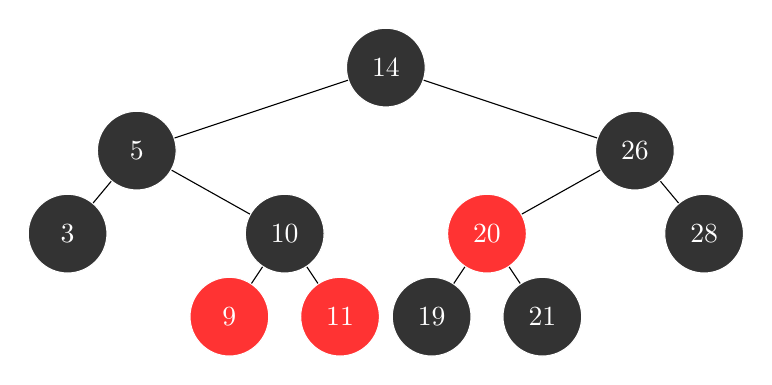
\begin{tikzpicture}
            \node[B]{14}
            child{
                node[B]{5}
                child{node[B]{3}}
                child{
                    node[B,xshift=10mm]{10}
                    child{node[R]{9}}
                    child{node[R]{11}}
                }
            }
            child{
                node[B]{26}
                child{
                    node[R,xshift=-10mm]{20}
                    child{node[B]{19}}
                    child{node[B]{21}}
                }
                child{node[B]{28}}
            };
        \end{tikzpicture}
    \end{center}
    \item \ 
    \begin{center}
        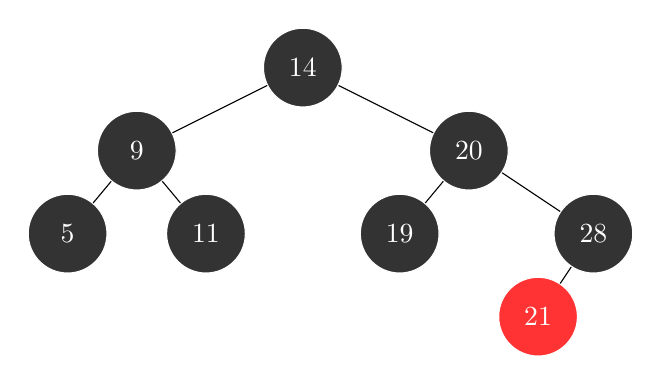
\begin{tikzpicture}
            \node[B]{14}
            child{
                node[B,xshift=3em]{9}
                child{node[B]{5}}
                child{node[B]{11}}
            }
            child{
                node[B,xshift=-3em]{20}
                child{
                    node[B]{19}
                }
                child{
                    node[B,xshift=2em]{28}
                    child{node[R]{21}}
                    child[missing]{}
                }
            };
        \end{tikzpicture}
    \end{center}
    \item Consider the following operation: Insert 4, insert 8, insert 7, insert 6 and delete 6. Then the red black tree is 
    \begin{center}
        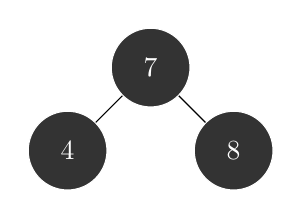
\begin{tikzpicture}
            \node[B]{7}
            child{node[B,xshift=6em]{4}}
            child{node[B,xshift=-6em]{8}};
        \end{tikzpicture}
    \end{center}
    This tree cannot be constructed using only insert. Since the node is initially red when it inserted into the tree.
    If this node do not violate the red-black properites, its color has remained red. Simply, for all $6!$ permutation of 
    \[
        \left\{\textup{insert } 4,\textup{insert } 8,\textup{insert } 7\right\},
    \]
    there is at most one node with red color, hence it cannot be constructed by only using insert.

    
    
    
\end{enumerate}

\end{document}
